\documentclass[13pt,a4paper]{extreport}
\usepackage[utf8]{inputenc}
\usepackage[utf8]{vietnam} %Bien dich duoc tieng Viet
\usepackage{amsmath,amsfonts,amssymb} %Font toan
\usepackage{type1cm}
\usepackage{graphicx}
\usepackage{subfig}
\graphicspath{ {images/} }
\usepackage[unicode]{hyperref} %Tu dong tao bookmark
\usepackage{indentfirst} %Thut vao dau dong o tat ca cac doan
\usepackage{listings} %Dinh dang code
\usepackage{color} %Mau sac
\usepackage[left=3.5cm,right=2.5cm,top=2.5cm,bottom=2.5cm]{geometry} %Canh lề trái - phải - trên - dưới cho tài liệu
\definecolor{dkgreen}{rgb}{0,0.6,0}
\definecolor{gray}{rgb}{0.5,0.5,0.5}
\definecolor{mauve}{rgb}{0.58,0,0.82}

\lstset{frame=tb,
  language=bash,
  aboveskip=3mm,
  belowskip=3mm,
  showstringspaces=false,
  columns=flexible,
  basicstyle={\small\ttfamily},
  numbers=left,
  numberstyle=\tiny\color{gray},
  keywordstyle=\color{blue},
  commentstyle=\color{dkgreen},
  stringstyle=\color{mauve},
  breaklines=true,
  captionpos=t,
  breakatwhitespace=true,
  tabsize=2
}
\begin{document}
%\input{title-page.tex}
\newpage

\pagenumbering{roman}


\tableofcontents

\newpage
\listoffigures
 
%\newpage
%\listoftables

\newpage
\pagenumbering{arabic}
\setcounter{page}{1}
\part{Một số dịch vụ lưu trữ đám mây trên Ubuntu}
%cloud computing
\chapter{Grive}
%Tai lieu tham khao: https://www.howtoforge.com/tutorial/sync-documents-with-google-drive-on-ubuntu-linux/
\section{Giới thiệu về Grive}
\begin{list}{--}{}
\item Với hệ điều hành Ubuntu, bạn không sử dụng được ứng dụng \verb|Google Drive| như trên hệ điều hành Windows, Mac hoặc Android mà thay vào đó chúng ta sử dụng ứng dụng \verb|Grive|.
\item \verb|Grive| có thể được tải bằng mã nguồn hay bằng gói \verb|deb|.
\item Trong bài viết này, mình chọn cách cài đặt ứng dụng \verb|Grive| bằng mã nguồn.
\end{list}
\section{Cài đặt Grive}
\begin{list}{--}{}
\item[] Gõ các lệnh sau:
\begin{lstlisting}[language=bash]
$ sudo apt-add-repository ppa:nilarimogard/webupd8
$ sudo apt-get update
$ sudo apt-get install grive
\end{lstlisting}
\end{list}
\section{Thiết lập tài khoản người dùng Grive}\label{Sec:setting-grive}
\begin{list}{--}{}
\item Đầu tiên, tạo một thư mục mà bạn muốn động bộ hóa lên Grive khi làm việc sau này: Có thể làm theo cách dưới -- tạo liên kết kết biểu tượng đến thư mục cần lưu.
\begin{lstlisting}[language=bash]
$ ln -s /path/ Grive
\end{lstlisting}
\begin{list}{+}{}
\item Với \verb|/path/| là đường dẫn đến thư mục cần lưu dữ liệu sau này khi cần đồng bộ, ví dụ \verb|/media/minhnhut/Data/Girve/|. %(ta nên chọn lưu trong ổ cứng để tiết kiệm dung lượng hệ thống và dễ dàng cho việc chia sẽ dữ liệu sau này).
\item Sau này khi thao tác, ta chỉ cần thao tác thư mục \verb|Grive| trong \verb|/home/minhnhut/|
\end{list}
\item Chạy lệnh bên dưới để liên kết đến tài khoản \verb|gmail| sử dụng \verb|Drive|: 
\begin{lstlisting}[language=bash]
$ grive -a
\end{lstlisting}
\begin{list}{+}{}
\item Click chuột phải vào đường link, chọn \verb|Copy Link Address|, dán địa chỉ vào trình duyệt web để liên kết đến tài khoản \verb|Gmail|.
\item Xuất hiện giao diện như hình \ref{Fig:Allow-grive}, click chọn \verb|Allow|.
\item Copy lại mã code mà \verb|gmail| thông báo như hình \ref{Fig:code-grive}, để dán vào của sổ \verb|Terminal| như hình \ref{Fig:use-code-grive}, rồi nhấn \verb|Enter| để xác nhận:
\begin{figure}[!h]
\begin{center}
\subfloat[Click chọn \textsf{Allow}\label{Fig:Allow-grive}]
	{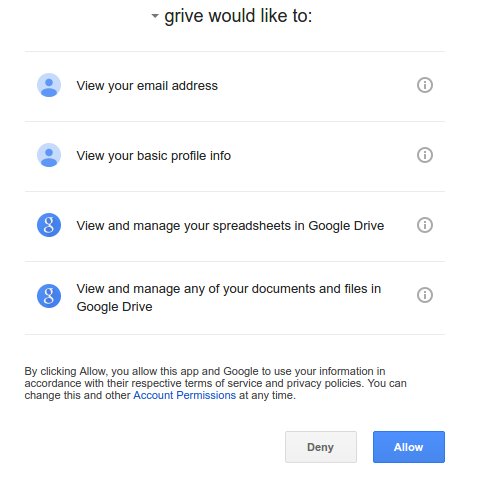
\includegraphics[scale=.43]{images/Allow-grive.png}}\\
\subfloat[Copy lại mã code \label{Fig:code-grive}]
	{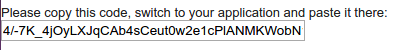
\includegraphics[scale=.6]{images/code-grive.png}}\\
\subfloat[Dán mã code vào của sổ \textsf{Terminal} \label{Fig:use-code-grive}]
	{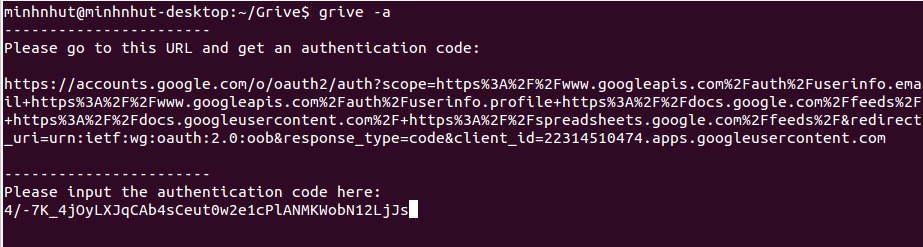
\includegraphics[scale=.4]{images/use-code-grive.png}}\\
	\subfloat[Kết nối đến tài khoản \textsf{gmail} sử dụng \textsf{Grive} thành công \label{Fig:succ-grive}]
	{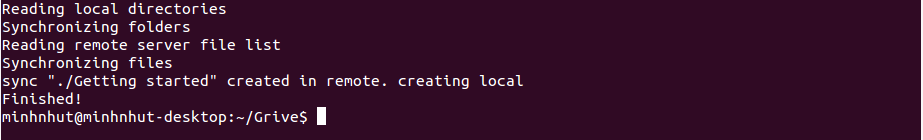
\includegraphics[scale=.4]{images/succ-grive.png}}\\
\end{center}
\caption{Cho phép liên kết đến tài khoản sử dụng Grive}
\end{figure}
\end{list}
\end{list}
\section{Đồng bộ dữ liệu với Grive}
\begin{list}{--}{}
\item Sau khi đã thực hiện bước cài đặt ở mục  \ref{Sec:setting-grive}, ta không cần phải đăng nhập lại mỗi khi đồng bộ.
\item Sử dụng lệnh sau để đồng bộ dữ liệu lên \verb|Google Drive|:
\begin{lstlisting}[language=bash]
$ grive sync
\end{lstlisting}
\item Kiểm tra những gì mà \verb|Grive| đã đồng bộ lên:
\begin{lstlisting}[language=bash]
$ grive --dry-run
\end{lstlisting}
\end{list}
\section{Các lệnh của ứng dụng Grive}
\begin{list}{--}{}
\item[] Các lệnh mở rộng với \verb|Grive|:
\begin{lstlisting}[language=bash]
Grive options:
  -h [ --help ]         Produce help message
  -v [ --version ]      Display Grive version
  -a [ --auth ]         Request authorization token
  -p [ --path ] arg     Path to sync
  -s [ --dir ] arg      Subdirectory to sync
  -V [ --verbose ]      Verbose mode. Enable more messages than 
                        normal.
  --log-http arg        Log all HTTP responses in this file for 
                        debugging.
  --new-rev             Create new revisions in server for updated 
                        files.
  -d [ --debug ]        Enable debug level messages. Implies -v.
  -l [ --log ] arg      Set log output filename.
  -f [ --force ]        Force grive to always download a file from 
                        Google Drive instead of uploading it.
  --dry-run             Only detect which files need to be 
                        uploaded/downloaded, without actually 
                        performing them.
  --ignore arg          Ignore files relative paths of which match 
                        this Perl 
                        RegExp.
  -m [ --move ] arg     Syncs, then moves a file (first argument) to                                     
                        new location (second argument) without 
                        reuploading or redownloading.

\end{lstlisting}
\end{list}
%\chapter{GitHub}
\end{document}